%%%%%%%%%%%%% You can ignore this stuff
\documentclass[bsc]{abdnthesis}
\usepackage[T1]{fontenc}
\usepackage[utf8]{inputenc}
\usepackage{booktabs}
\usepackage{longtable}
\usepackage{csquotes}
\usepackage{minted}[linenos, breaklines]
\usepackage{url}
\usepackage{pdflscape}

\usepackage[style=apa, backend=biber]{biblatex}
\DefineBibliographyStrings{english}{%
  bibliography = {References},
}
\addbibresource{library.bib}

% This creates hyperlinks and moves the contents links to the page number for clarity
\usepackage[linktocpage=true,hidelinks]{hyperref}	

\def\subsectionautorefname{Section}
\def\subsubsectionautorefname{Section}
\def\sectionautorefname{Section}
\def\chapterautorefname{Chapter}

%%%%%%%%%%%%%%%%% Space for your own packages here %%%%%%%%%%%%%%%%%%%%%%%%%%%%%%
% Uncomment for blank lines between paragraphs rather than
% indents
\usepackage[parfill]{parskip}

%%%%%%%%%%%%%%%%%%%%%%%%%%%%%%%%%%%%%%%%%%%%%%%%%%%%%%%%%%%%%%%%%%%%%%%%%%%%%%%%%

\title{Using AI to Predict Bangladesh's Drinking Problem}
\author{Kane Swartz}
\upnumber{941226}

\projecttype{Research Project}
\school{School of Computing}

%%%% In the final submission of a thesis, this should only be the year
%%%% of submission.  However, it is useful to use \date{\today} for drafts so that
%%%% they don't get mixed up.
    
\date{2023}

%% It is useful to split the document up as chapters and include
%% them.  LaTeX will sort out all the numbering and cross-referencing
%% for you --- if you run it enough times!

\begin{document}

%%%% Create the title page and standard declaration.

\maketitle
\makedeclaration

%%%% Then the abstract and acknowledgements

\begin{abstract}
  An expansion of the title and contraction of the thesis.
\end{abstract}

\begin{acknowledgements}
  Much stuff borrowed from elsewhere
\end{acknowledgements}

%% please indicate whether you are happy for other students to
%% view your project in the future
\section*{Consent to Share}
I consent for this project to be archived by the University Library and potentially used as an example project for future students.

%%%% These are macros ( each macro is defined by \newcommand )
%%%% These macros make cross-referencing easier, building on the
%%%% already very useful \autoref{ref}.  You tweak them or build your own.

%% \autorefp{ref}
%% Like \autoref, but adds the page number
%% e.g. Section 3.2.4 (p345)
\newcommand{\autorefp}[1]{\autoref{#1} (p\pageref*{#1})}

%% \autorefnp{ref}
%% Like \autoref, but adds both the section name and page number
% e.g. Section 3.2.4 "blah blah" (p345)
\newcommand{\autorefnp}[1]{\autoref{#1} ``\nameref{#1}'', (p\pageref*{#1})}

%% \see{ref}
%% Handy shorthand for inserting a hyperlinked xref.
%%   e.g. (see Section 3.2.4, p134)
%%        (see Figure 5.1, p23)
%%        (see Table 4.7, p999)
\newcommand{\see}[1]{\hyperref[#1]{(see \autoref*{#1}, p\pageref*{#1})}}

%% \seenamed{ref}
%% Handy shorthand for inserting a hyperlinked xref that also includes
%% the name of the section being referred to.
%% (see Section 3.2.4 "blah blah", p134)
%% (see Figure 5.1 "blah blah blah!", p23)
%% (see Table 4.7 "blah blah blah blah blah blah", p999)
\newcommand{\seenamed}[1]{\hyperref[#1]{(see \autoref*{#1} ``\nameref*{#1}'', p.\pageref*{#1})}}

%% \bq Block Quotations.
\newcommand{\bq}[2][]{\singlespacing \begin{quote} 
\begin{small} ``\textit{#2}'' \end{small} #1 \end{quote} \doublespacing}

%% \qq{quotation}
%% Shortcut for doing inline quotations (with 6699 quotation marks around italic text)
%% e.g. \qq{To be, or not to be}
\newcommand{\qq}[1]{{\enquote{\textit{#1}}}}

%%%% It should have a table of contents, but delete the other two as
%%%% necessary.

\tableofcontents
\listoftables
\listoffigures

\chapter{Introduction}

\section{Background and Historical Context}

Arsenic pollution in groundwater is a problem faced worldwide \parencite{khan2014groundwater}. Southeast Asian populations, particularly those of Bangladesh, are arguably the most negatively impacted by arsenic contamination in drinking water worldwide. 

This is largely due to the use of tube wells, many of which were built as a result of the United Nations Children's Fund (UNICEF) working with the Bangladeshi government from 1970 to provide safe drinking water to 80\% of the population by the year 2000 \parencite{Smith2000}. 

These tube wells were typically installed at a depth of under 200 meters. Arsenic concentrations in groundwater peak at between 15 and 25 meters of depth and are typically only below the World Health Organisation's safe arsenic limit of 10$\mu$g/litre \parencite{WHO2003} at 200 meters of depth or more \parencite{Chakraborti2010}. 

Prior to the discovery of harmful levels of arsenic in the water from these tube wells, their installation was acclaimed as a huge success with regards to providing the population with clean drinking water \parencite{khan2014groundwater}. Tubewells today are still extremely popular in Bangladesh with approximately 95\% of rural people and 70\% of urban people using them in 2020 \parencite{Ghosh2020}.

\section{Solution Approach}

- The exact nature of this problem is highly complex

- To overcome the issue, there is no one solution, rather, multiple solutions which each tackle an aspect of the problem

Sub issues to tackle

- providing access to safe drinking water

- Education about drinking water and the negative health impact of polluted water, often people find it hard to believe water that appears clear can be dangerous / linked to disease

- Medical treatment for those affected (just those who have developed disease such as cancer or those with acute arsenic poisining? Find citations arguing those points)

- Policy and government changes such as aiming for comprehensive testing of wells and the disabling of polluted wells and provision of an alternative source, where there is no source it would only cost \$x to deepen the well to a safe level

- Humanitarian engagement with communities to ensure cooperation with practices designed to mitigate exposure (ie not using a well that's been confirmed as polluted) 

\section{What is iArsenic}

iArsenic is a web application that estimates the arsenic concentration for a well in Bangladesh based on its geographic region, depth and visible staining on the well.

This is achieved by aggregating source data about these wells and using that aggregate data to produce expert system prediction models which are available on the web page.

The tooling developed to produce these models are general-purpose and modular, enabling them to be imported into other projects. The time and expertise required to clean and aggregate the source data are very substantial and leveraging this existing work allows higher-level outcomes to be brought into scope.

The data in iArsenic has been selected from reputable sources and represents a large and high-quality dataset, representing the majority of Bangladesh.
\chapter{Literature Review}

\section{Existing Work}

The existing iArsenic model uses a decision tree developed by a human expert, as opposed to by a machine learning algorithm. This approach has the benefit of the output of the model being explainable and justifiable.

Talk about existing works using various techniques:

- geospatial mapping

- Hydrogeochemical modeling

- groundwater monitoring

- field screening techniques such as testing wells

- machine learning techniques using data gathered from methods above

Explain pros and cons of each

\section{The Black Box Problem}

(Fleming et al 2021) states that acceptance of machine learning based approaches have faced resistance in earth \& environmental sciences due to the inability to explain how machine learning models are working and the lack of understanding of artificial intelligence within the earth \& environmental sciences field. While this is partially true in terms of the black box problem there is are numerous of examples of machine learning techniques being utilized to analyze groundwater quality. A more difficult question to answer is whether these models are less applicable in real life compared to human designed models, though in machine learning it is often asserted as common knowledge that this is the case (Guidotti et al, 2018).

In machine learning, the black box problem is based on the inability to explain how a model works, or more specifically, how a model produces an output for any given input.

To illustrate why this is an issue \cite{Castelvecchi2016} uses the following thought experiment. Imagine a black box machine learning model was created with a set of images of mammograms including labels indicating whether the person in the scan went on to develop breast cancer. It could happen that this model out performs human medical professionals in predicting whether someone would go on to develop breast cancer.

One could argue that the benefit of this model would be that it could identify when women should have a preventative mastectomy. However, critics assert that critical decisions cannot be made without justification and that one cannot justify a decision that cannot be explained (Loyola-Gonzalez, 2019). The human doctor's opinion will always be explainable.

Not all machine learning algorithms produce models considered to be black box systems. Decisions tree style models for example are powerful machine learning tools which produce models considered white box systems meaning you can analyse them to determine how they're working \parencite{Caruana2006}. Decision tree style models can be contrasted with neural network style models, the latter of which is only not considered a black box system in exceptional circumstances, due to the complex nature of neural networks.

Because determining whether a drinking water source is safe or not does factor into critical decision making, it is important to explore the black box problem. The purpose of this project however, is simply to compare a the accuracy of a predictive model developed with machine learning to an existing model designed by an expert. Therefore whether a model is black box or white box will not come into consideration during model selection and design though this will be reflected on later.

\section{Tool Selection}

%why sci-kit learn over TensorFlow - tensorflow is primarily used for deep learning mention focus on quick prototyping to asses the potential for more complex models to be implemented (using tensorflow)

\section{Model Type}

The initial steps in model selection are rudimentary. Broadly speaking machine learning algorithms fall into three categories, supervised learning, unsupervised learning and reinforcement learning. Because our data set consists of structured and labelled data the appropriate choice is supervised learning.

Furthermore, in order to have a comparable evaluation metric to the existing model we have to select a model with a comparable output. The existing model outputs a classification of safe, polluted or highly polluted. This indicates that we should select a classification algorithm. 

In Géron A's book, Hands-On Machine Learning with Scikit-Learn (Géron, 2017), it is noted that some regression algorithms can be used for classification, and vice versa. However because the iArsenic data set is highly nominal, containing no quantitative features before feature engineering the data is not well suited to typical regression algorithms.

Thus we have narrowed our algorithm search to supervised learning, classification algorithms.

Rich Caruana and Alexandru Niculescu-Mizil provide a comparison of a number of supervised learning algorithms on a range of data sets and performance measures (Caruana C., Niculescu-Mizil A., 2006). We have chosen algorithms the following algorithms based on their performance and availability within the tools we have access to.

The algorithms we will be basing our models on are as follows: Support Vector Machines (SVMs), K-Nearest Neighbours (KNN), Random Forests (RFs) and Decision Trees (DTs).

\section{Experiment Methodology}

When designing and conducting experiments with predictive models, 

\subsection{Data Cleaning}

\subsection{Validation}

\subsection{Model Performance}

\subsection{Evaluation Methods}

While regression models are typically evaluated based on the difference between a predicted value and the actual value, classification models are evaluated primarily on the misclassification rate; how often the model predicts the correct class opposed to the incorrect class.

The following evaluation metrics have been selected where they apply to both the machine learning model and the existing model.

In a binary classifier classification accuracy can be presented as a confusion matrix to find the false positive and false negative rate among predictions. As the existing model uses multi-class classification, these classes being, safe, polluted and highly polluted, we will not be evaluating the false positive and false negative values for the model as a whole. We can however display a confusion matrix for each output class as in this way each class can be presented as a binary classification.

Additionally we can evaluate the null accuracy of the model by calculating the accuracy if the model always produces the same output. This provides a good baseline from which we can determine if the model is actually producing useful outputs.

We will also evaluate the misclassification rate of the models. This is a measure of how often the classifier makes an incorrect prediction.

The sensitivity, a measure of how often the prediction is correct when the value is positive, the specificity, how often the prediction is correct when the value is negative will also be evaluated.

%\^\^ cite this whole section with chapter 3 of hands on machine learning with scikit learn and also https://www.ritchieng.com/machine-learning-evaluate-%classification-model/ if possible

- talk about managing the size of the feature space, calculate how big it could be with our dataset and how big it can reasonably be




\chapter{Methodology}

% TODO reference why this is being referred to as agile via the agile manifesto
% TODO reference gannt chart in PID in appendix
At the start of the project a high level representation of the research and development steps required to complete the project was created. Theses steps were allocated a time frame and a sprint was planned at the start of each time frame.

While each sprint was different, sprints broadly involved defining a clear goal and pursuing it until the end of the sprint window. While the sprint windows were not strict cut offs, the primary focus of my time would change upon the start of a new sprint window.

% TODO bottom two paragraphs can come at the top
This workflow is best described as a modified agile scrum methodology with a variable and flexible sprint window for each objective.

This chapter will chronologically outline the steps planned and taken in the progression of the project.

% TODO reference this to PID use agile to explain why headings / steps changed

% TODO as well as chapter intro include chapter conclusion
\section{Steps Taken}

\subsection{Research Potential Projects}

The first step in this project was to identify potential project ideas. This was done with brainstorming, both by thinking about the project and talking about it with others.

The project ideas broadly fell into two categories, engineering, where the objective is to produce an application, and research, where the objective is to provide insight or an answer to an unknown.

A personal goal for me in this project was to develop my skills in machine learning and artificial intelligence. Evaluating the iArsenic models and producing alternative models with machine learning appealed to me as the most exciting option. Additionally, because the project already contained hours of existing work, the objectives of the project could build off this work instead of starting from scratch. This enabled higher level and higher impact objectives to be set. 

As Dr Mohammed Hoque agreed to be the client to this project I was able to commit to this project, confident in knowing it had purpose and direction from the client.

\subsection{Clarify the Project Objectives}

Originally the vision of the project was to develop machine learning based models and compare their performance to the existing iArsenic models.

This initial vision is however does not define several key aspects of the project. How does one evaluate the performance of an iArsenic model? How does this compare to an evaluation of a machine learning based model? What is the purpose of developing new models and comparing them to the existing ones?

Ultimately the desired outcomes were clearly defined as follows:

% TODO desired outcomes could probably live somewhere else
\textbf{Desired Outcomes}

\begin{enumerate}
  \label{desired_outcomes}
  \item To evaluate the existing models
  \item To compare the performance of the existing models with typical machine-learning-based models
\end{enumerate}

Desired Outcome 1 was requested from the client. Evaluating the models informs the client of how each iteration of the models have impacted their performance and, because this model is deployed, verifies the quality of the predictions being made in deplyoment.  While the existing models were developed with expert knowledge, prior to the evaluations conducted in this project, the performance of the models was unknown.

The purpose of desired outcome 2 comes from \cite{Fleming2021}'s assertion that machine learning should be part of Earth and Environmental Science (EES). iArsenic provides an opportunity for a case study where expert system models can be compared to supervised learning models. 

It is difficult to ascertain what level of sophistication of machine learning models an EES graduate would reasonably be able to implement.  Because supervised learning algorithms are standardised in scikit-learn, this project suggests that these models are the kind that an EES graduate with approximately 2 undergraduate modules of machine learning could implement.

\subsection{Research Applied Machine Learning Methodologies}

To design implement and evaluate machine learning models for iArsenic, I first had to research machine learning to understand what specific areas in machine learning could be applied to this dataset to achieve the desired outcomes of the project and then had to develop these models in code to gain the practical experience required.

Chapter 2 of \cite{Aurélien2017}'s book Hands-On Machine Learning with Scikit-Learn and TensorFlow was the primary resource for breaking through the barrier of theoretical knowledge, gained from written sources such as \cite{Caruana2006} which compares several supervised machine learning models in different applications, to actually producing my own implementations of these models.

% TODO, could all the code in this section be moved to experiment design
\subsection{Understanding the iArsenic Codebase}

The iArsenic codebase provided the following key functions:

\begin{enumerate}
  \label{ia_functions}
  \item Producing a standard dataset
  \item Generating iArsenic models from a dataset
  \item Generating predictions from these generated models
\end{enumerate}

By looking at the iArsenic website and know it produced a model based on existing data which could produce a prediction for a given data point, it was clear that the project included this functionality.

To learn how to achieve this functionality, I would read the iArsenic code in GitHub and experiment with it as an npm package.

\textbf{Producing a standard dataset}

The iArsenic script csv-to-json.js makes exporting a standardised dataset trivial.

This function is implemented in the project via an package script:

\begin{figure}[h]
\begin{minted}[linenos, breaklines]{json}
"scripts": {
    "load-src-data": "mkdir well_data ; node node_modules/preprocessing/preprocessing/cli/csv-to-json.js -p node_modules/preprocessing/data/*.csv -o well_data/src_data.json",
\end{minted}
\label{fig:x load_ia_data}
\caption{package.json snippet showing script to load data from iArsenic}
\end{figure}

See the file at \url{https://github.com/portsoc/iArsenic/blob/master/preprocessing/cli/csv-to-json.js}

\textbf{Generating iArsenic models from a dataset}

To verify that a model can generalise to new cases, it must be trained on a subset of the data and tested on a separate subset of data which it has not been previously exposed to. In the iArsenic webapp, the models are trained on the entire source dataset. See \ref{fig:x imp_iam_webapp} on page \pageref{fig:x imp_iam_webapp} for an flowchart showing this implementation.

Generating the models on a training subset of the data was done by passing 4 of the 5 subsets of the data, after the data was split into 5 for k-folds cross validation, to the iArsenic model generator. This was done for each of the 5 subsets of the data for each of the 3 iArsenic models. See \ref{fig:x programmatically_gen_ia_model} on \pageref{fig:x programmatically_gen_ia_model} to see the code that achieved this.

\begin{figure}[h]
    \centering
    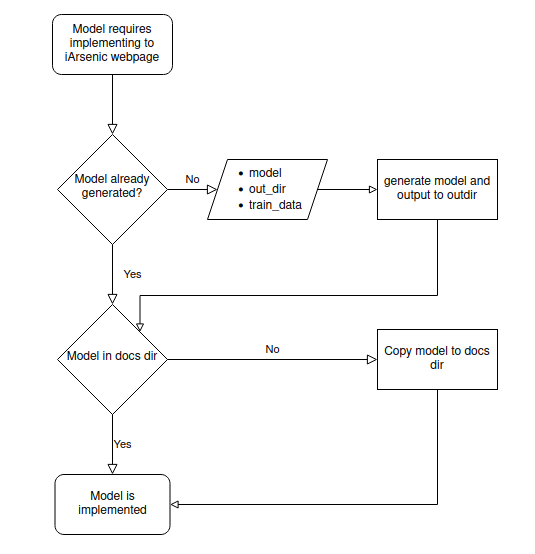
\includegraphics[scale=0.6]{figures/implement_ia_model_to_webapp.png} 
    \caption{Flowchart showing process to implement model in iArsenic webapp}
    \label{fig:x imp_iam_webapp}
    \small The code that generates the models can be found at: \url{https://github.com/portsoc/iArsenic/blob/master/preprocessing/cli/produce-aggregate-data-files.js}
\end{figure}

\begin{figure}[h]
    \begin{minted}[linenos, breaklines]{python3}
def gen_model(train_src, out_dir, model):
  if not os.path.exists(out_dir):
    os.mkdir(os.path.join(out_dir))

  cmd = [
    'node',
    'node_modules/preprocessing/preprocessing/ cli/produce-aggregate-data-files.js', 
    '-m',
    model,
    '-o',
    out_dir,
    '-p',
    train_src,
    'node_modules/preprocessing/data/mouza-names.csv',
  ]
  stdout = check_output(cmd).
    decode(sys.stdout.encoding).
    replace('\n', '')
    
  print(stdout)
      \end{minted}
    \caption{Python code used to programmatically generate iArsenic models}
    \label{fig:x programmatically_gen_ia_model}
\end{figure}

\textbf{Generating predictions from generated iArsenic models}

The web application index.html file shows a script.js file is used, in this file a global function called produceEstimate is called from the estimator.js script. See \ref{fig:x produce_estimate_call} on \pageref{fig:x produce_estimate_call} to see this function call.

Comments in the estimator.js file indicate that this file is a component of the generated model. Therefore this function is used as a generic entry point for producing estimates for each model. Because model5 requires a parameter containing Mouza regional data to be but model3 and model4 do not, the implementation of this function call depends on the model being used. See \ref{fig:x programatically_gen_ia_predictions} page \pageref{fig:x programatically_gen_ia_predictions} to see this dual implementation.

\begin{figure}
    \begin{minted}[linenos, breaklines]{python3}
    const estimate = produceEstimate(aggregateData, inputs.division, inputs.district,
      inputs.upazila, inputs.union, inputs.mouza, inputs.depth, inputs.colour, inputs.utensil, inputs.flooding);
    \end{minted}
    \caption{Code used in iArsenic to produce estimate from a model in the webapp}
    \label{fig:x produce_estimate_call}
    \small The file containing this code can be found at: \url{https://github.com/portsoc/iArsenic/blob/master/docs/script.js#L340-L341}
\end{figure}

\subsection{Developing New Models}

To familiarise myself with implementing machine learning models, I initially followed the tutorial in Chapter 2 of \cite{Aurélien2017}'s book Hands-On Machine Learning with Scikit-Learn. I then implemented 4 separate supervised learning models on 25 datasets.

\begin{landscape}
    \begin{figure}[h]
        \centering
        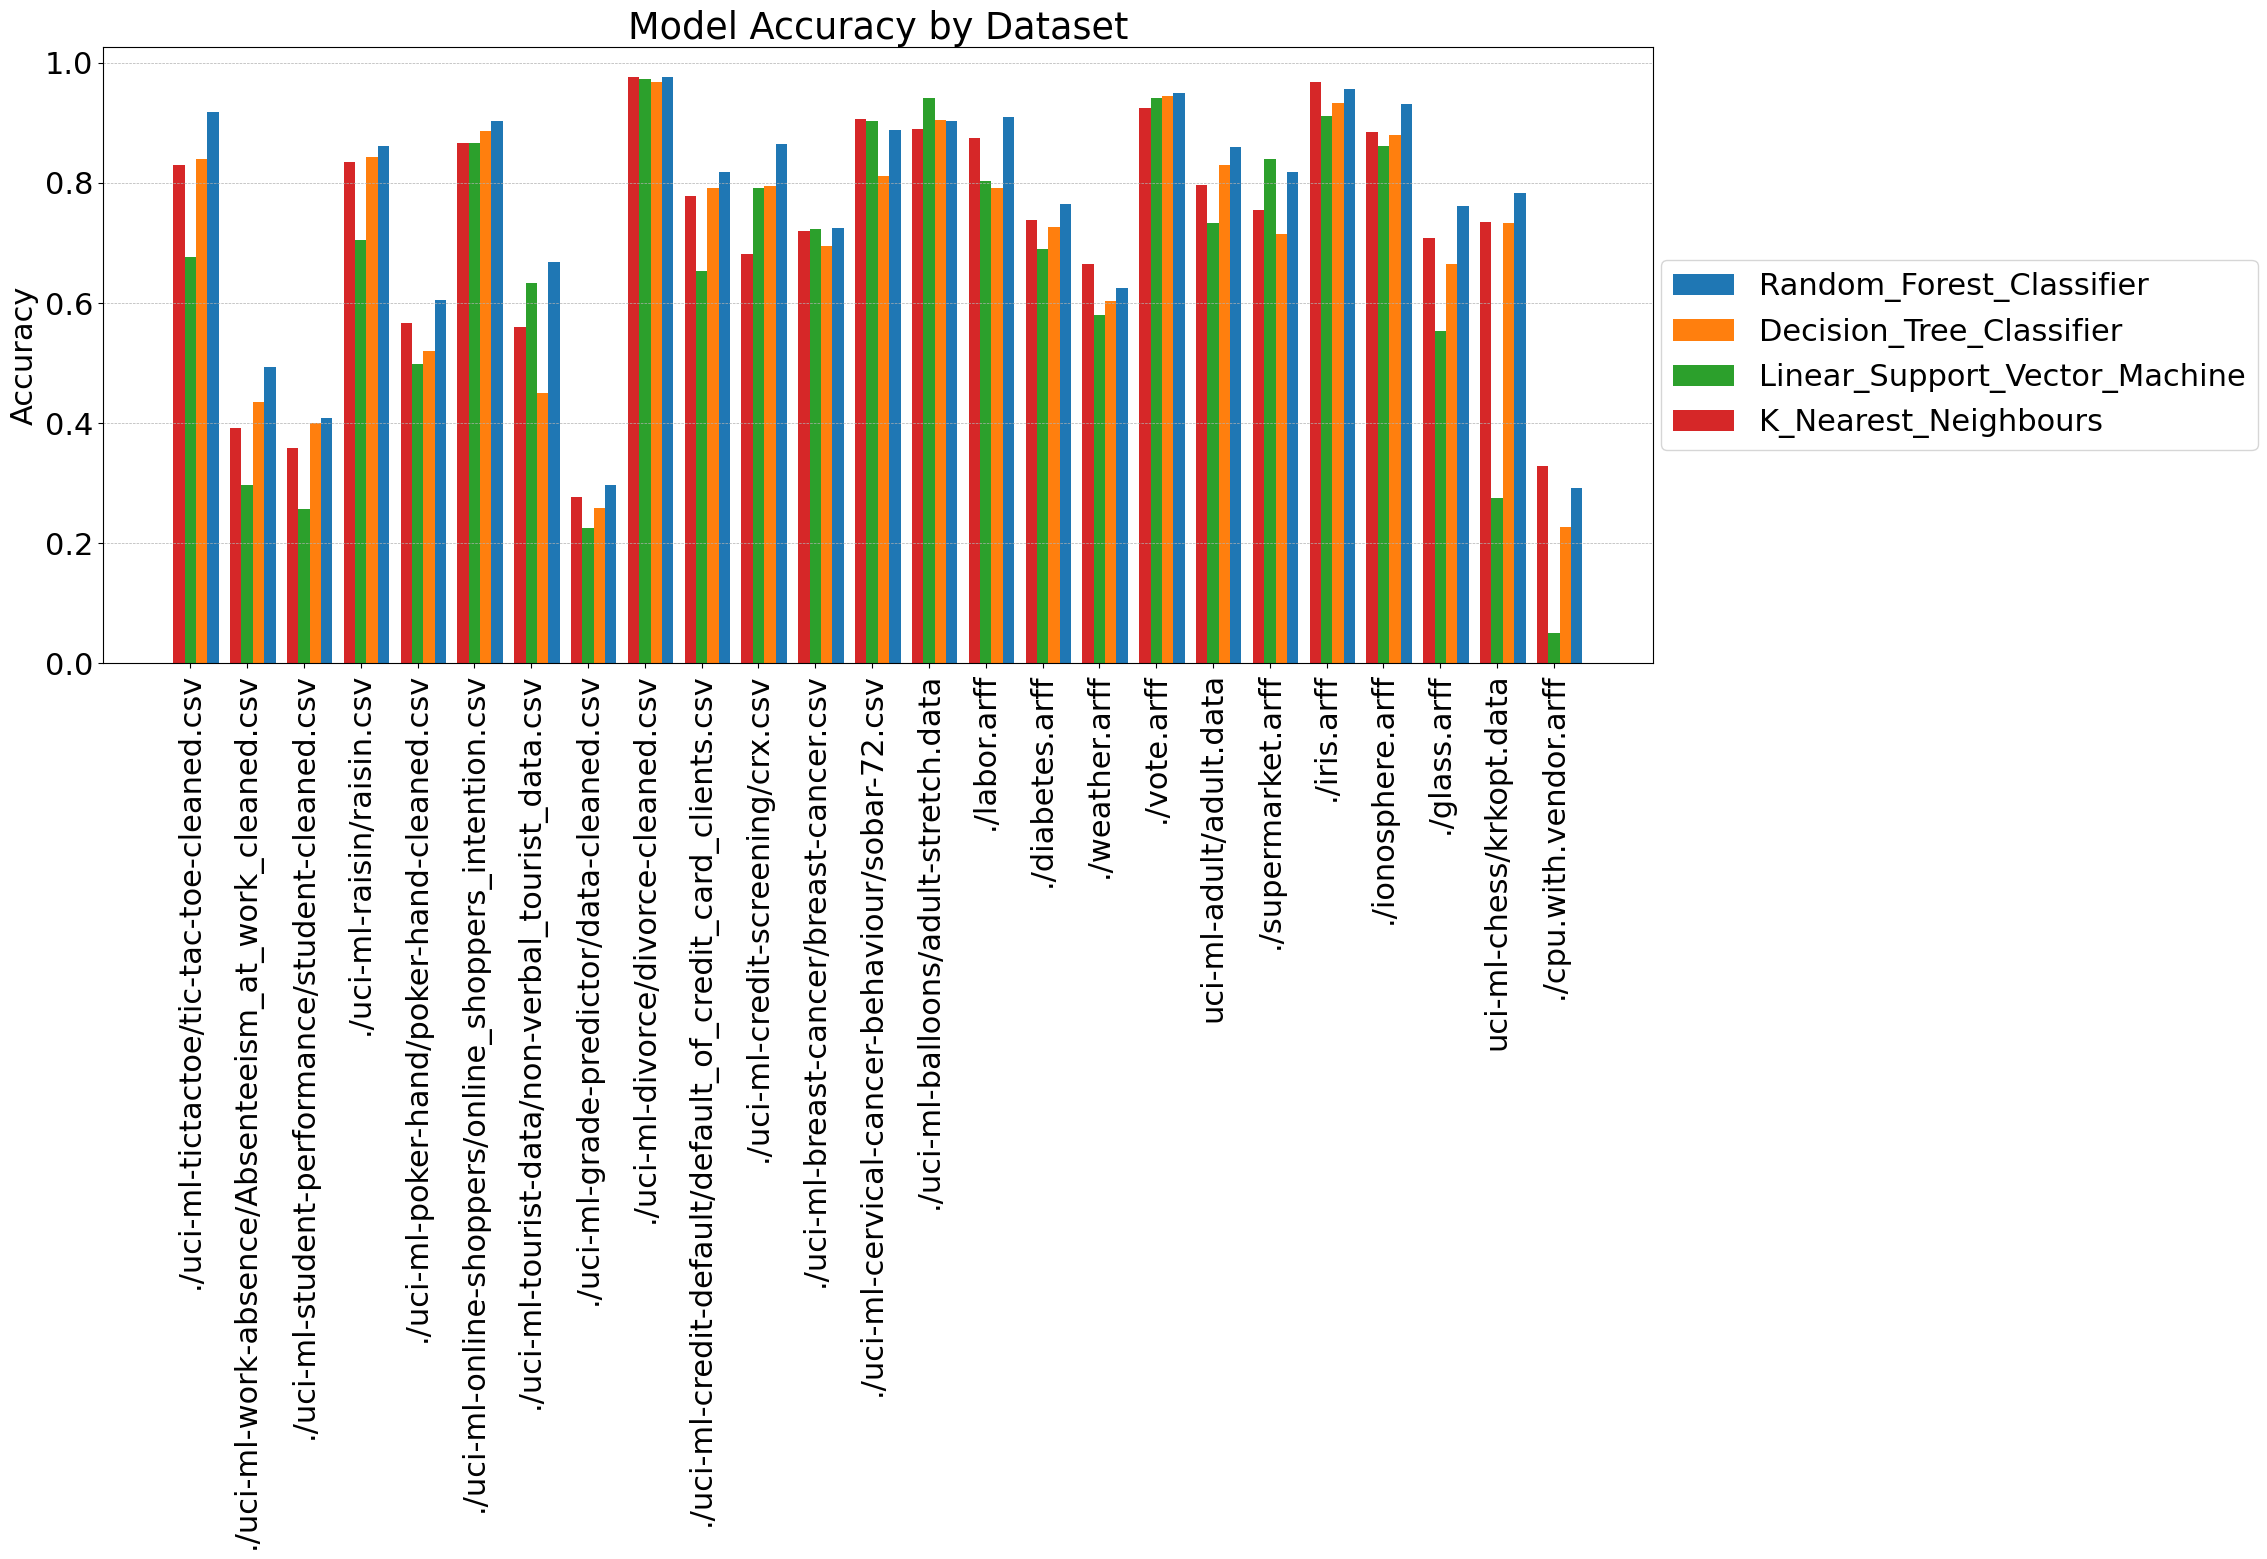
\includegraphics[scale=0.375]{figures/4_models_25_datasets.png} 
        \caption{Summary of results of supervised model implementation practice}
        \label{fig:x 4_m_25_d}
    \end{figure}
\end{landscape}

\subsection{Integrating iArsenic and scikit-learn}

The prototype implementations of both iArsenic and machine learning based models allowed each model to take input data and produce estimations individually. 

Because it takes multiple days to run every experiment required, it is not practical to have a human run each model individually, as the time taken between an experiment finishing and the next starting will depend on when the person gets around to it. By making the models run programmatically this is not an issue. It also allows the project to be more portable, allowing it to be run on a remote server or high performance computer.

To run both NodeJS based iArsenic models and Python based scikit-learn models an integration layer between Python and NodeJS had to be created. Python was chosen as the main program to run the NodeJS code from as a personal preference. Using NodeJS would also have been a reasonable choice.

The iArsenic models are run from Python by passing data over the storage drive as CSV files. See function gen\_ia\_predictions in \ref{fig:x py_call_node} which calls the script containing the code snippet in figure \ref{fig:x programatically_gen_ia_predictions}, passing a filepath to a CSV file of datapoints and reading the CSV returned from the NodeJS script which generated a CSV file containing predictions for the datapoints passed, for a specified iArsenic model.

\begin{figure}[h]
    \begin{minted}[linenos, breaklines]{Python}
def gen_ia_predictions(test_src, stain_color, model, k_fold):
  cmd_arr = [
    'node',
    './models/model_utils/iarsenic-wrapper.js',
    test_src,
    stain_color,
    model,
    str(k_fold),
  ]

  stdout = check_output(cmd_arr).decode(sys.stdout.encoding).replace('\n', '')
  df = pd.read_csv(stdout)
  
  df['Prediction'].replace('highlyPolluted', 'polluted', inplace=True)
  df['Prediction'].replace('We do not have enough data to make an estimate for your well', 'polluted', inplace=True)

  return df['Prediction']
        \end{minted}
    \caption{Python script used to call NodeJS script which produces predictions for an iArsenic model}
    \label{fig:x py_call_node}
\end{figure}

\begin{figure}[h]
    \begin{minted}[linenos]{javascript}
  const estimate = (() => {
    if (model === 'model5') {
      return produceEstimate(
        divisions,
        div,
        dis,
        upa,
        uni,
        mou,
        depth,
        colour,
        utensil,
        flood
      );
    } else {
      return produceEstimate(
        divisions,
        div,
        dis,
        upa,
        uni,
        depth,
        colour,
        utensil
      );
    }
  })()
      \end{minted}
    \caption{NodeJS code which will generate a prediction for a datapoint from a passed CSV file. This code is run for each row of the CSV file.}
    \label{fig:x programatically_gen_ia_predictions}
\end{figure}



\chapter{Experiment Design}

This chapter defines how the desired outcomes defined in the Methodology will practically be met. This requires describing the available code and data, how it will integrate with new code developed in this project and what the new code being developed is.

Additionally, this chapter describes existing work and data to the reader.

\subsection{Well Data in iArsenic}

The data used by iArsenic can be found in the CSV in the data/ directory of iArsenic (note that this does not include CSV files in sub-directories of the data/ directory). These files have been selected on the following criteria for aggregating:

\begin{itemize}
    \item two CSV files do not include the same datapoint
    \item the CSV contains standard features required by the iArsenic models
\end{itemize}

Before preprocessing, these files contain 1,144,586 rows (including headers) combined.

The primary preprocessing function provided by iArsenic is name correcting. This is the process of renaming region names such that a region with different names in different datasets, has the same name in an aggregate dataset. These corrections allow the well data and the geodata to be aggregated. Most name differences are caused by differences in phonetic translation or inconsistent capitalisation.

After preprocessing, the iArsenic data source contains 868,679 rows (including headers).

See figure \ref{fig:x avg_datapoints} on page \pageref{fig:x avg_datapoints} for a choropleth of datapoints per District.

\begin{figure}[!htb]
    \centering
    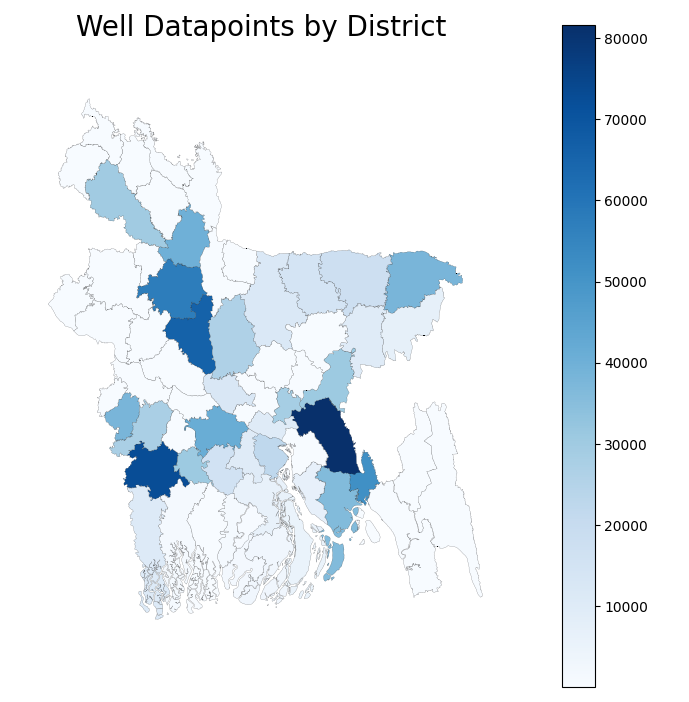
\includegraphics[scale=0.6]{figures/data_distribution_by_district.png} 
    \caption{Distribution of Well Data by District in iArsenic Processed Dataset}
    \label{fig:x avg_datapoints}
\end{figure}

The attributes included in the aggregate data file output by iArsenic are the following:

\begin{itemize}
    \item Division
    \item District
    \item Upazila
    \item Union
    \item Mouza
    \item Depth
    \item Arsenic
\end{itemize}

Excluding Depth and Arsenic, these attributes are all region names with corresponding geographic data. 

See figure \ref{fig:x labelled_divisions} on page \pageref{fig:x labelled_divisions} for a labelled map of Bangladesh divisions.

\begin{center}
    \begin{tabular}{|c c c c|} 
         \hline
         Name & Mean Area $km\textsuperscript{2}$ & Mean Area $\sigma$ & Unique Values \\ [0.5ex] 
         \hline\hline
         Division & 17,482 & 6,928 & 8 \\ 
         \hline
         District & 2,185 & 1,080 & 63 \\
         \hline
         Upazila & 257 & 185 & 445 \\
         \hline
         Union & 27 & 41 & 2,838 \\
         \hline
         Mouza & 2.4 & 8.4 & 9,550 \\ [1ex] 
         \hline
    \end{tabular}
\end{center}

\begin{figure}
    \centering
    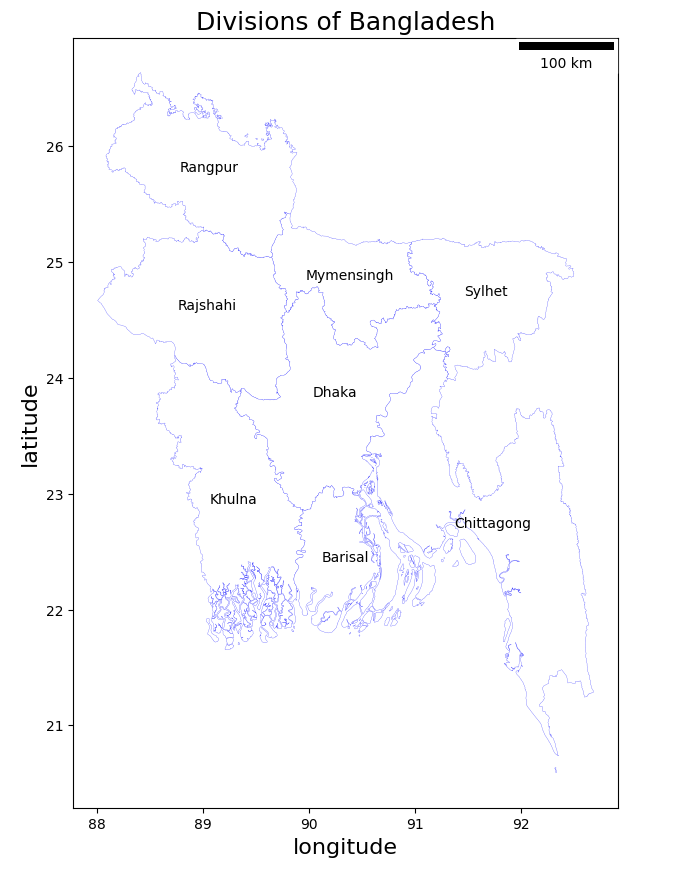
\includegraphics[scale=0.6]{figures/labelled_divisions.png} 
    \caption{The regions of Bangladesh as per the iArsenic dataset}
    \label{fig:x labelled_divisions}
\end{figure}

\textbf{Depth}

The Depth column refers to the depth of a well in meters.

The deepest well in the dataset is 445 meters, the lowest is 0, the is mean 40 meters and the standard deviation is 52 meters. See figure \ref{fig:x avg_depth} on page \pageref{fig:x avg_depth} for a choropleth of mean depth per Upazila.

\begin{figure}[!htb]
    \centering
    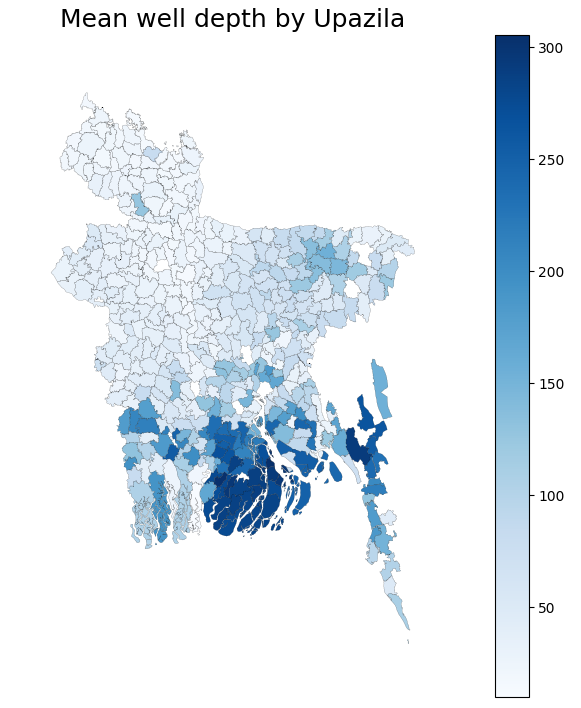
\includegraphics[scale=0.6]{figures/mean_well_depth_by_upa.png} 
    \caption{Average (mean) Well Depth by Upazila}
    \label{fig:x avg_depth}
\end{figure}

\textbf{Arsenic}

The Arsenic column refers to the arsenic concentration in water from a well datapoint in micrograms per litre ($\mu$g/l).

The highest concentration of arsenic in the dataset is 4,000$\mu$g/l (4ng/l), the lowest concentration of arsenic is 0$\mu$g/l, the mean is 41$\mu$g/l and the standard deviation is 74$\mu$g/l. See figure \ref{fig:x avg_as} on page \pageref{fig:x avg_as} for a choropleth of mean depth per Upazila.

\begin{figure}[!htb]
    \centering
    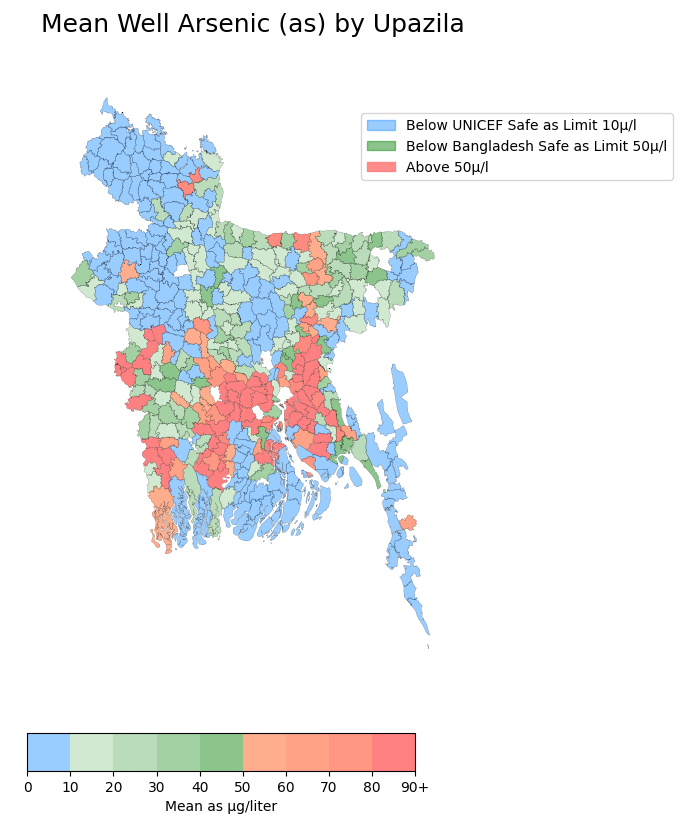
\includegraphics[scale=0.6]{figures/mean_as_by_upazila.png} 
    \caption{Distribution of Average (mean) Arsenic by Upazila in Preprocessed iArsenic Dataset}
    \label{fig:x avg_as}
\end{figure}

\newpage

\textbf{Why use this Dataset?}

While new and existing iArsenic models could be trained on different data, the time and resources required to produce a dataset of this quality and suitability are substantial and outside the scope of this project. 

\subsection{Geodata}

The original source of the geodata is unclear, though similar country based polygon data can be found on the first page of google.

% reference where these instructions are in iArsenic
The geodata has been zipped and added to the project's repository using Git Large File Storage. This is because some of the geodata is omitted from the original iArsenic repository due to it exceeding the GitHub file size limit. Instructions are provided in iArsenic for regenerating this missing data.

\section{iArsenic Integration}

\subsection{Data Preparation}

The iArsenic code repository is downloaded from GitHub via Node Package Manager (npm). This repository includes selected source data and several tools to process this data.

% TODO reference csv-to-json script in appendix
Data is extracted from iArsenic using the csv-to-json.js script. This script aggregates the source files into a single data structure and outputs it as a JSON file. Additionally, it ensures that all regions follow the same naming convention, which is essential because it prevents distinct data points in the same region from appearing to be in two different regions. This enables the data to be matched to its corresponding polygon in the geodata.

% TODO reference the utils/src_to_test_train.py script and the generated files
The JSON file is then converted to a pandas DataFrame in Python, shuffled to ensure there is no ordering bias, and converted into 5 separate CSV files. It is split into 5 to enable k-fold cross-validation on the dataset.

These 5 CSV files are what we use to test and train the models.

\subsection{Generating the iArsenic Models}

iArsenic can generate 3 separate models: model3, model4 and model5.

Originally an iArsenic model was generated on all available data and then made available on the iArsenic webpage. Due to their modular design however, the models can also be imported into NodeJS code.

To evaluate the models using k-folds cross-validation, each of the 3 models was generated 5 times with 4 of the CSVs used for training and 1 for testing, thus implementing k-folds cross-validation. This generated a total of 15 iArsenic models.

\subsection{Interfacing With Generated iArsenic Models}

% TODO reference iarsenic-wrapper.js
% TODO explain that the ia models generate multiple classifications but have been simplified to safe or not safe
Predictions are generated from the generated model using a NodeJs wrapper script. This will be referred to as the iArsenic Model Wrapper

The predictions are saved to a temporary CSV file and the name of this file is logged to the standard output.

The wrapper script requires the following parameters to be passed as system arguments:
\begin{itemize}
  \item a CSV file containing the data points to use to generate predictions
  \item the stain colour of the well the data point is from
  \item the model to generate the prediction from
  \item the k-fold version of the model to generate the prediction from
\end{itemize}

Initially, the wrapper script would produce an estimate from one data point at a time, passed as a system argument. However, this took more time than pracitcal to process when passing the test dataset. Therefore the test dataset is passed as a CSV filepath.

% TODO specify what is the source data, maybe have raw data, source data and kfolds data
% TODO link to section in evaluation
% TODO include a chart showing the performance with different colours for models34&5

\subsection{Imputing Stain Colour}

In the original iArsenic webpage, the stain colour was to be specified by a user entering parameters about a real well, allowing the user to observe and provide the staining colour of the well. The data extracted from iArsenic however did not include staining colour data. 

When working with missing values there are primarily 3 options: 

% TODO reference handson ml scikit learn here
\begin{enumerate}
    \item remove the feature with missing values
    \item delete all rows containing missing data
    \item replace missing data with a fixed value
\end{enumerate}

Because the iArsenic models will not run with the colour omitted, option 1 is not viable. Because none of the rows contain staining data, option 2 is also not viable. Therefore we must fill in the data with a fixed value, either 'Red' or 'Black'.

To determine whether the value should be set to 'Red' or 'Black', the models have been evaluated using each and the value with which the model performs best, 'Red', has been selected. Figure \ref{fig:x ia_model_black_red_accuracy} on page \pageref{fig:x ia_model_black_red_accuracy} shows the accuracy of the iArsenic models with 'Black' or 'Red' used as the imputed well colour.

\begin{figure}[h]
    \centering
    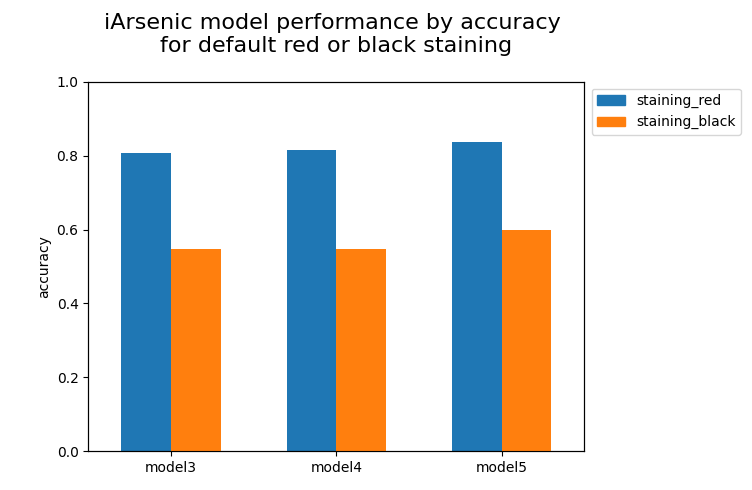
\includegraphics[scale=0.55]{figures/ia_model_black_red_accuracy.png} 
    \caption{iArsenic model performance by accuracy for default red vs black staining}
    \label{fig:x ia_model_black_red_accuracy}
\end{figure}

\newpage

% TODO maybe reference the number of positives and negatives in the original dataset
Considering the accuracy score alone, it would appear that setting the parameter to 'Red' produces the best model performance by approximately 10\%. A higher accuracy score however does not guarantee that one model outperforms another. This could happen because the source data has a much higher positive than negative rate and the model always predicts positive for example. Therefore specificity and sensitivity must also be considered.

Comparing the sensitivity and specificity of the models shows that when the staining is set to 'Black' model3 and model4 always assume the well is safe. The sensitivity, the true positive rate, becomes 0 and the specificity, the true negative rate, becomes 1. Occasionally model5 will classify black staining as polluted but the specificity is effectively 0. While the specificity is lower when the staining is set to 'Red', the sensitivity is much higher for each model, indicating better performance.

\newpage

\begin{figure}[!htb]
    \centering
    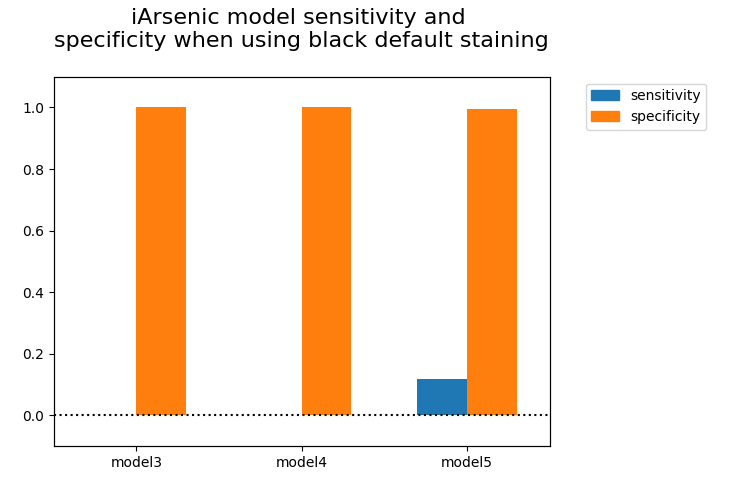
\includegraphics[scale=0.55]{figures/ia_models_sensitivity_vs_specificity_black.png} 
    \label{fig:x ia_svs_black}

    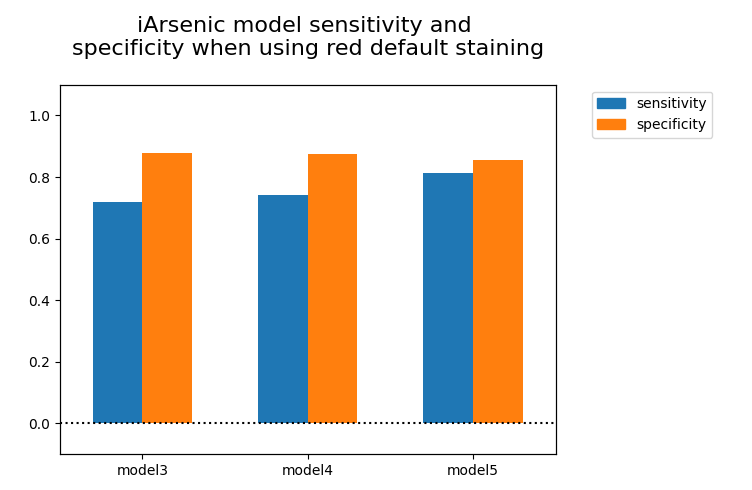
\includegraphics[scale=0.55]{figures/iarsenic_model_sensitivity_vs_specificity_red.png} 
    \caption{Model sensitivity and specificity stain parameter 'Black' (top) vs 'Red' (bottom)}
    \label{fig:x ia_svs_red}
\end{figure}

\newpage

Generating two confusion matrices for model5, one generated from 'Black' passed as a parameter and one from 'Red', reinforces the conclusion that using 'Red' as a parameter produces a better model.

\begin{figure}[!htb]
    \centering
    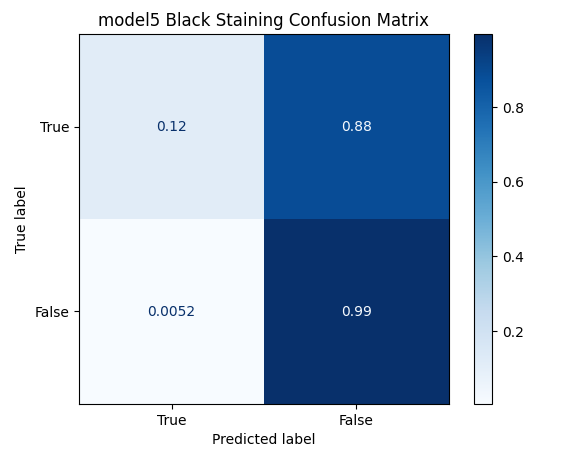
\includegraphics[scale=0.6]{figures/m5_black_cm.png} 
    \label{fig:x Confusion Matrix mode5 Black Staining}
    
    \centering
    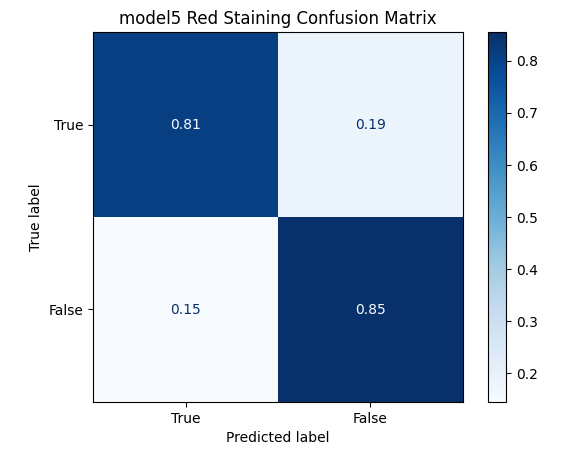
\includegraphics[scale=0.6]{figures/m5_red_cm.png} 
    \caption{Confusion Matrix model5 'Black' (top) vs 'Red' (bottom) Staining}
    \label{fig:x Confusion Matrix mode5 Red Staining}
\end{figure}

\newpage

\textbf{Qualitative Approach to Selecting Staining Parameter}

Observing the evaluation metrics of the iArsenic models and comparing them when producing predictions with either 'Red' or 'Black' as the staining parameter has indicated that the models perform better with 'Red' passed as a parameter. This is however still arguably down to interpretation.

A qualitative comparison of the models, using a value such as Area Under the Curve (AUC) would be preferable. This however is not possible with the iArsenic models as there is no feature to change the classification threshold, which is required to generate a Receiver Operating Curve (ROC) and therefore calculate AUC.

\section{Generating the Machine Learning Models}

The machine learning models are made with scikit-learn in Python. 

Each model is defined in an individual Python script and exported as a Python module.

\section{Creating a Common Model Interface}

The machine learning models will be made in Python. These can be interfaced with directly using Python modules with parameters passed directly into function calls. This is inconsistent with the iArsenic models which are run via the iArsenic wrapper with node, passing parameters using command line arguments.

A Common Module Interface has therefore been specified which standardises how the modules should be interacted with. This interface specifies that each model will have a main function which takes two parameters, the test data source and the k-fold number and rehouseturns predictions as a pandas dataframe. Each model can be run via a Python module that follows this standard.

\subsection{Implementing the Common Model Interface}

% TODO display some kind of figure or diagram of the file structure, possibly a generic and an example
Each model has a directory in the top level models directory. Each model directory contains a model.py file which exports a Python module which can generate predictions based on the Common Module Interface, in addition to any other resources required by the model.

% TODO reference gen_predictions in ia_model_wrap.py
The iArsenic Model Wrapper cannot accept variables passed by Python. Therefore a Python to NodeJS Bridge has been created. The Python to NodeJS Model Bridge works by running the iArsenic Model Wrapper from Python in a subprocess managed by Python.

The Python to NodeJS Bridge can then be imported to the top level main.py script.

\section{Evaluating the Models}

% TODO refer to these terms explained in the literature review, not explained in this e
The predictions returned from the common model interface are used for evaluation. The follow evaluation metrics are generated:
\begin{itemize}
  \item accuracy (\(\frac{true\_positives + true\_negatives}{total\_predictions}\))
  \item sensitivity (\(\frac{true\_positive}{true\_positive + false\_negative}\))
  \item precision (\(\frac{true\_positive}{true\_positive + false\_positive}\))
  \item specificity (\(\frac{true\_negative}{true\_negative + false\_positive}\))
  \item f1 score (\(\frac{precision * sensitivity}{precision + sensitivity}\))
\end{itemize}

\section{Creating a Main Script to Run \& Evaluate Experiments}

The Common Module Interface allows the models imported to the main.py script and run programmatically, without specific code defined for each model. 

This facilitates maintainable code as the complexity of the code increases. The complexity of the main.py script necessitates steps to ensure maintainability are taken. 

Significant complexity has been introduced in making the models run and build concurrently. This is important however as doing this sequentially would take more time than is practical.

While the iArsenic models benefit the most from being run concurrently, as these are single threaded, so running them concurrently allows more of the host machine's CPU power to be utilised by using multiple CPU cores.

The machine learning models however are written using scikitlearn libraries, which are able to use all CPU cores available. 

Further optimizing the models by, for example, running the iArsenic models concurrently and the machine learning models sequentially was not deemed necessary, as building and running all models concurrently took approximately 3.5 days, which is a practical amount of time. This run was achieved on a server computer with Ubuntu 22.01, an 8 x 1.8GHz core CPU and 96GB 1600MHz DDR3 RAM.

\subsection{Main Script Structure}

The purpose of the main.py script is to provide an entrypoint to execute all required steps of the project.

The main script takes the following steps:
\begin{enumerate}
    \item extract the iArsenic \& geodata
    \item generate the k-folds cross-validation data split 
    \item build the iArsenic models
    \item generate predictions from all models
    \item generate an evaluation for each model's predictions
\end{enumerate}

\section{Development of New Models}

%Introduction to the process taken for each model, hypothesizing why a hypothetical model would work then explaining the preprocessing required and implementation.

%- models are developed using typical supervised learning models like RF KNN 

%- regression models are not used as the purpose of the models is to compare with the existing iArsenic models which are classification 

\subsection{model6}

Model6 is an implementation of scikit-learn's random forest classifier with the default configuration.

Because this model cannot process string values, all string values are converted to numerical values, with each new string given an identification number in ascending order.

\subsection{model7}

model7 is also a default implementation of scikit-learn's random forest classifier. This model incorporates computed region attributes computed in model5.

model5 uses feature engineering to calculate the median, lower quartile and upper quartile of the arsenic in a region, for a given depth range.

The hypothesis is that this feature engineering will provide the model with information that correlates with the model prediction target for a given datapoint, improving the models performance.

These values are therefore incorporated into the dataset used for model7. Where the values for a region are missing from the model5 dataset, the values from the region's parent are used.

\subsection{model8}

model8 uses a feed forward neural network, scikit-learn's MultiLayer Perceptron Classifier (MLPClassifier) model.

\textbf{Neural Network Configuration}

\begin{center}
    \begin{tabular}{|c c c c|} 
         \hline
         Hidden Layers & Solver & Learning Rate & Epochs \\ [0.5ex] 
         \hline\hline
         3 & adam & adaptive & 100 \\ 
         \hline
    \end{tabular}
\end{center}

The first hidden layer consists of half the number of inputs, the next hidden layer one quarter the number of inputs and the final hidden layer one eighth. The adam algorithm is used because it is generally faster than standard gradient descent on datasets this size. An adaptive learning rate is used to allow the performance to increase up to the maxiumum limit of 100 epochs.

\textbf{Data Preprocessing \& Feature Engineering}

The median, upper quartile and lower quartile arsenic values are imported from the model5 processed data to the dataset used by this model.

The smallest region size, the Mouzas are one hot encoded, allowing each Mouza to have a corresponding input node.

The region columns are dropped.

The data is normalised between 0 and 1.

\textbf{Model Optimization}

Due to the number of Mouzas (9550), the model could not allocate enough memory to run with the source data passed directly.

Therefore the source data has been split into 8 subsets by Division (See figure \ref{fig:x labelled_divisions} on page \pageref{fig:x labelled_divisions}. For each Division a model is trained with the datapoints within that region and predictions are generated. These predictions are then added to their corresponding datapoints in the source dataset.

The mechanism of this optimization can be seen in figure \ref{fig:x m8_code} on page \pageref{fig:x m8_code}.

\begin{figure}[h]
    \begin{minted}[linenos]{python3}
      for div in train_df['Division'].unique():
        tr_div = train[train['Division'] == div]
        te_div = test[test['Division'] == div]
    
        tt_df = append_test_train(te_div, tr_div)
    
        conv_cat_num(tt_df, 'Label')
        tt_df = ohe_col(tt_df, ['Mouza'])
    
        tt_df = tt_df.drop(
          columns=[
            'Division',
            'District',
            'Union',
            'Upazila',
          ]
        )
    
        cat_int_enc(tt_df)
        tt_df = pd.DataFrame(
          MinMaxScaler().fit_transform(tt_df), 
          columns=tt_df.columns
        )
    
        te_div, tr_div = split_test_train(tt_df)
    
        train_X = tr_div.drop(['Arsenic', 'Label'], axis='columns')
        train_y = tr_div['Label']
        test_X = te_div.drop(['Arsenic', 'Label'], axis='columns')
    
        num_feat = len(test_X.columns)
    
        clf = MLPClassifier(
          solver='adam',
          alpha=0.0001,
          hidden_layer_sizes=(
            math.trunc(num_feat / 2), 
            math.trunc(num_feat / 4), 
            math.trunc(num_feat / 8)
          ),
          learning_rate='adaptive',
          random_state=99,
          max_iter=100,
        )
    
        clf.fit(train_X, train_y)
    
        test.loc[test['Division'] == div, ['Prediction']] = clf.predict(test_X)
    \end{minted}
    \caption{Snippet showing m8 optimization method, where a different model is trained for each of the 8 Divisions}
    \label{fig:x m8_code}
\end{figure}

\subsection{model9}

model9 is also based on scikit-learn's MLPClassifier.

\textbf{Neural Network Configuration}

\begin{center}
    \begin{tabular}{|c c c c|} 
         \hline
         Hidden Layers & Solver & Learning Rate & Epochs \\ [0.5ex] 
         \hline\hline
         2 & adam & adaptive & 100 \\ 
         \hline
    \end{tabular}
    % TODO add label / caption to the table
\end{center}

The first hidden layer consists of 50 nodes, the next hidden layer consists of 2 nodes. An adaptive learning rate is used to allow the performance to increase up to the maxiumum limit of 100 epochs.

\textbf{Data Preprocessing \& Feature Engineering}

The source data is merged with the geodata and each datapoint is attributed with a latitude and longitude. All other feature columns are dropped.

\subsection{model10}

model10 uses scikit-learn's of the k-nearest neighbors classification algorithm, the KNeighborsClassifier. The number of neighbours is set to 50.

\textbf{Data Preprocessing \& Feature Engineering}

The source data is merged with the geodata and the latitude and longitude of each Mouza is attributed to each datapoint. All other feature columns are dropped.

This model will find the 50 datapoints with the smallest difference in terms of latitude, longitude and depth in the training set then make a prediction from the classification of these datapoints.

\subsection{model11}

Like model10, model11 uses scikit-learn's implementation of the k-nearest neighbours classification algorithm. The number of neighbours is set to 250.

\textbf{Data Preprocessing \& Feature Engineering}

This model uses the data processed by model5, including the lower median and upper quartile arsenic values for a region.

This model will find the 250 datapoints with the smallest difference in median, lower quartile and upper quartile values of arsenic in the training dataset and make a prediction from the most common classification of those nearby datapoints.
\chapter{Results and Evaluation}

In section \ref{desired_outcomes} on page \pageref{desired_outcomes} the desired outcomes of the project are described. This chapter critically assesses to what extent these outcomes have been met.

\section{Evaluating the Existing Models}


\include{conclusion}
\chapter{Reflection \& Future Work}

- utilize flooding data in a model

- develop ensemble model with base models trained on training k-split 

- deep learning model approach using convolutional neural networks

- improvements to existing models such as ensuring proper test train split where not applicable in current setup

- NEAT based model

- Neural network pruning

- Evaluating the iarsenic models on limited datasets to evaluate the application space of expert models in this area

- Area Under the Curve analysis on iArsenic models
\chapter{References}

Bindal, S., \& Singh, C. K. (2019). Predicting groundwater arsenic contamination: Regions at risk in highest populated state of India. Water research, 159, 65-76.\\

Caruana, R., \& Niculescu-Mizil, A. (2006, June). An empirical comparison of supervised learning algorithms. In Proceedings of the 23rd international conference on Machine learning (pp. 161-168).\\

Castelvecchi, D. (2016). Can we open the black box of AI?. Nature News, 538(7623), 20.\\

Connolly, C. T., Stahl, M. O., DeYoung, B. A., \& Bostick, B. C. (2021). Surface flooding as a key driver of groundwater arsenic contamination in Southeast Asia. Environmental Science \& Technology, 56(2), 928-937.\\

Chakraborti, D., Rahman, M. M., Das, B., Murrill, M., Dey, S., Mukherjee, S. C., ... \& Quamruzzaman, Q. (2010). Status of groundwater arsenic contamination in Bangladesh: a 14-year study report. Water research, 44(19), 5789-5802.\\

Connolly, C. T., Stahl, M. O., DeYoung, B. A., \& Bostick, B. C. (2021). Surface flooding as a key driver of groundwater arsenic contamination in Southeast Asia. Environmental Science \& Technology, 56(2), 928-937.\\

Fleming, S. W., Watson, J. R., Ellenson, A., Cannon, A. J., \& Vesselinov, V. C. (2021). Machine learning in Earth and environmental science requires education and research policy reforms. Nature Geoscience, 14(12), 878-880.\\

Géron, A. (2017). Hands-on machine learning with scikit-learn and tensorflow: Concepts. Tools, and Techniques to build intelligent systems.\\

Ghosh, G. C., Khan, M., Hassan, J., Chakraborty, T. K., Zaman, S., Kabir, A. H. M., \& Tanaka, H. (2020). Human health risk assessment of elevated and variable iron and manganese intake with arsenic-safe groundwater in Jashore, Bangladesh. Scientific reports, 10(1), 1-9.\\

Guidotti, R., Monreale, A., Ruggieri, S., Turini, F., Giannotti, F., \& Pedreschi, D. (2018). A survey of methods for explaining black box models. ACM computing surveys (CSUR), 51(5), 1-42.\\

Khan, N. I., \& Yang, H. (2014). Arsenic mitigation in Bangladesh: An analysis of institutional stakeholders' opinions. Science of the total environment, 488, 493-504.\\

Loyola-Gonzalez, O. (2019). Black-box vs. white-box: Understanding their advantages and weaknesses from a practical point of view. IEEE Access, 7, 154096-154113.\\

Najafabadi, M. M., Villanustre, F., Khoshgoftaar, T. M., Seliya, N., Wald, R., \& Muharemagic, E. (2015). Deep learning applications and challenges in big data analytics. Journal of big data, 2(1), 1-21.\\

Smith, A. H., Lingas, E. O., \& Rahman, M. (2000). Contamination of drinking-water by arsenic in Bangladesh: a public health emergency. Bulletin of the World Health Organization, 78(9), 1093-1103.\\

Van Halem, D., Bakker, S. A., Amy, G. L., \& Van Dijk, J. C. (2009). Arsenic in drinking water: a worldwide water quality concern for water supply companies. Drinking Water Engineering and Science, 2(1), 29-34.\\

Winkel, L., Berg, M., Amini, M., Hug, S. J., \& Annette Johnson, C. (2008). Predicting groundwater arsenic contamination in Southeast Asia from surface parameters. Nature Geoscience, 1(8), 536-542.\\

World Health Organization. (2003). Arsenic in drinking-water: background document for development of WHO guidelines for drinking-water quality (No. WHO/SDE/WSH/03.04/75). World Health Organization.\\

%%%%%%%%%%%%%% REFERENCES SECTION
\newpage
\phantomsection
\addcontentsline{toc}{chapter}{References}
% In order to try and get a consistent format I copy and paste the INSPIRE bibtex code into my bibtex file.
\printbibliography

%%%%%%%%%%%% Include your appendices here

\appendix

\end{document}
